%!TEX root = ./presentation.tex

\begin{frame}{Inhalt}
	\begin{block}{}
		\begin{itemize}
			\item ...
		\end{itemize}
	\end{block}
\end{frame}

%-----------------------------------------------------------

\section{Algorithmen}
\begin{frame}
\begin{center}
\huge{\textbf{{\secname}}}
\end{center}
\end{frame}

%-----------------------------------------------------------
\begin{frame}{Lineare Interpolation}
\begin{figure}
  \centering
     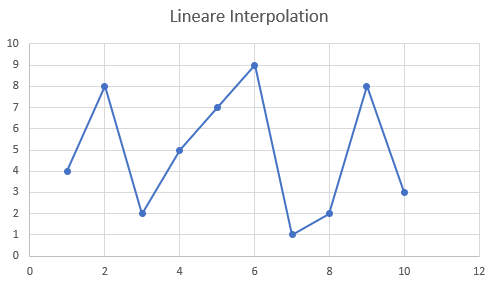
\includegraphics[width=0.5\textwidth]{pics/linear.png}
  %\tiny{\caption{Übersicht der Bestandteile}}
  \label{fig:Bild1}
\end{figure}
\begin{itemize}
\item Verfahren legt eine Gerade zwischen zwei Punkte $x_1$ \& $x_2$
\item Gesuchte Werte liegen auf der Geraden
\item Für jeden unbekannten Datenpunkt P(x/y) gilt:
$$y = y_1 + \frac{y_2 - y_1}{x_2 - x_1} \cdot (x - x_1)$$
mit $x1\leq\ $x $\leq \ x_2$
\item Erzeugt stetigen, aber keinen glatten Verlauf der Funktion
\end{itemize}
\end{frame}


%-----------------------------------------------------------
\subsection{Polynomielle Interpolationsverfahren}
\begin{frame}{\insertsubsectionhead}
\begin{figure}
  \centering
     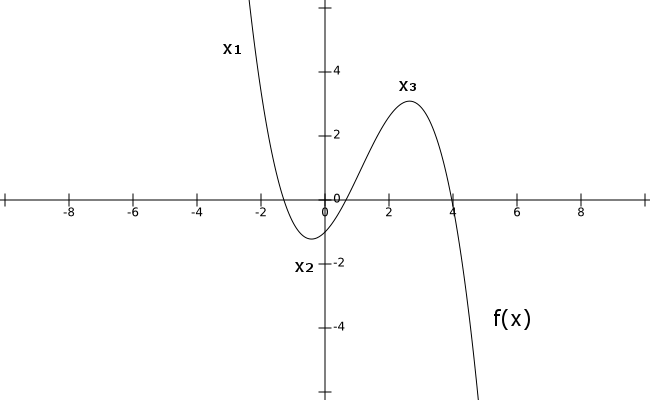
\includegraphics[width=0.7\textwidth]{pics/polynoms.png}
  %\tiny{\caption{Übersicht der Bestandteile}}
  \label{fig:Bild1}
\end{figure}
\begin{itemize}
\item Versuchen, durch gegebene Punkte eine Kurve zu legen
\item Finden zu n+1 paarweise verschiedenen Datenpunkten ein Interpolationspolynom maximal n-ten Grades
\end{itemize}
\end{frame}

%-----------------------------------------------------------
\begin{frame}{Interpolationsverfahren nach Newton (1/2)}
\begin{block}{Ziel des Algorithmus}
\begin{itemize}
\item Mathematische Erklärung folgt
\item 
\end{itemize}
\end{block}
\begin{block} {Algorithmus}
\underline{Vorteile}
\begin{itemize}
\item Bilden von dividierten Differenzen aus den n nächsten Nachbarn
\end{itemize}
\end{block}
\end{frame}

%-----------------------------------------------------------
\begin{frame}{Interpolationsverfahren nach Newton (2/2)}
\begin{block} {Charakteristika}
\underline{Vorteile}
\begin{itemize}
\item Polynom muss bei weiteren Punkten nicht komplett neu berechnet werden (vgl. Interpolation nach Lagrange)
\end{itemize}
\underline{Nachteile}
\begin{itemize}
\item Je größer der Grad, desto instabiler die Polynome (schwingen stark zwischen sehr verschiedenen Punkten)
\item \textit{Lösung:} Betrachtung der n nächsten Nachbarn
\end{itemize}
\end{block}
\end{frame}

%-----------------------------------------------------------
\begin{frame}{Splines}
\begin{block}{Ziel des Algorithmus}
\begin{itemize}
\item Finden von Stützstellen zwischen vorhandenen Datenpunkten
\item Jeder Teil des Splines ist durch eine Parabel mit geeigneten Koeffizienten definiert, z.B. $a_{i}x^3 + b_{i}x^2 + c_{i}x + d_{i}$
\begin{itemize}
\item Heraus kommt eine Funktion niedrigen Grades
\item Interpolation wird stückweise vorgenommen
\end{itemize}
\end{itemize}
\end{block}
\begin{block} {Charakteristika}
\underline{Vorteile}
\begin{itemize}
\item Linearer Rechenaufwand
\item Polynome werden nicht zunehmend instabiler
\end{itemize}
\underline{Nachteile}
\begin{itemize}
\item Können keine Verbrauchswerte in der Zukunft vorhersagen
\end{itemize}
\end{block}
\end{frame}

%-----------------------------------------------------------
\subsection{\glqq Intelligente\grqq Interpolationsverfahren}
\begin{frame}{\insertsubsectionhead}
text
\end{frame}


